\chapter{Charge pump regulation}
\section{Theory and related work} \label{sec:literature_chargepump}
A charge pump is a type of switching regulator that delivers power by alternatively charging and discharging capacitors and is specifically useful for supplying circuits with a low load current \cite{WebsiteChargePump}. Charge pumps are more efficient than linear regulators as there are no heat losses and can produce an inverting output by connecting the output to ground.

\section{Design} \label{sec:design_chargepump}
 The design of the charge pump circuit and switching transistor implemented is shown in \ref{fig:system_diagram}, here a maximum supply current of $\SI{5}{\milli A}$ was chosen.\newline The first step in designing the charge pump is deciding on a suitable charge tank capacitor $C_1$ that will ensure a continuous supply of current to the load. The larger the size of this capacitor the bigger the size of the maximum load. For the purpose of this design a $\SI{1}{\milli F}$ capacitor was chosen, and to remove any ripple voltages a $\SI{10}{\nano F}$ capacitor was placed in parallel with it. A secondary smaller capacitor $C_2$ had to be designed to discharge completely within the period of the $\SI{10}{\kilo Hz}$ pulse train to supply charge to the larger capacitor, here a low ESR $\SI{10}{\micro F}$ capacitor was chosen.\newline
 Since the square wave pulse train will be generated by an Arduino Beetle with a limited current supply an alternative current source had to be designed. For this purpose a common emitter configuration was chosen to provide a current gain to the output whilst providing no voltage gain, suitable collector and base resistors had to be designed such that the transistor could turn on and current could flow such as to charge up capacitor $C_2$.\newline A base resistor of $\SI{10}{\kilo \Omega}$ was chosen to minimize current losses through the transistor, and collector resistor of $\SI{200}{\Omega}$ was chosen to supply enough current to the $\SI{-5}{V}$ rail and small enough to ensure that the $\SI{625}{\milli W}$ maximum power rating of the transistor would not be exceeded.
 
 \begin{figure}
    \centering
    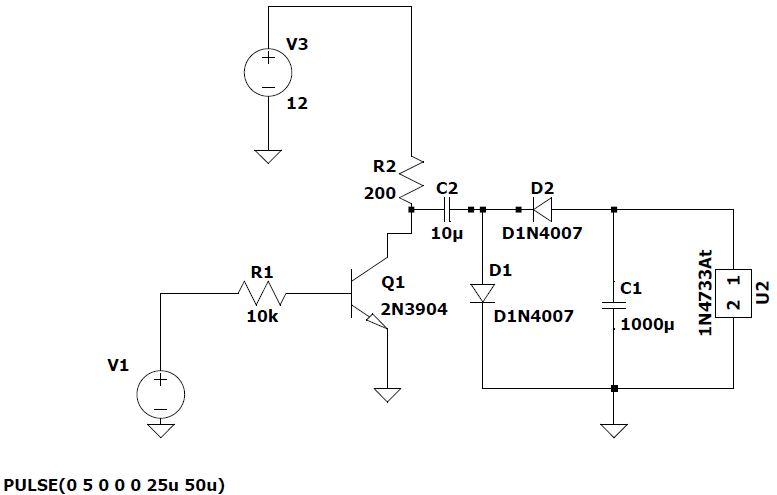
\includegraphics[width = 0.7\linewidth]{Figures/charge_pump_schem.JPG}
    \caption{Circuit Schematic of the $\SI{-5}{V}$ Regulator}
    \label{fig:charge_pump_design}
\end{figure}

\section{Simulation} \label{sec:simulation_chargepump}
After simulating the circuit in SPICE and testing it under various loads the output voltage was measured and tabulated in Table \ref{tab:chargepumptable}. It was found that a stable $\SI{-5}{V}$ could be supplied by the regulator under load conditions not exceeding $\SI{5}{\milli A}$, for load conditions exceeding this limit the supply voltage dropped drastically. \newline The theoretical efficiency of this charge pump circuitry was found by calculating the power dissipated in the load and summing all of the power into the charge pump and applying Equation \ref{eq:efficiency}. The regulator had an extremely low efficiency of $8.16\%$ and a half Watt rated resistor had to be chosen for the collector resistor. 

\begin{table}
        \centering
        \footnotesize
        \caption{Table showing simulated voltage output of charge pump.}
         \begin{tabular}{c@{\qquad}rrrr}
          \toprule
           Load Resistance ($\Omega$) & Output Voltage ($\SI{}{V}$)) \\
           \midrule
            No load         & 4.9989 \\
            10k             & 4.9959 \\
            4.7k            & 4.9923 \\
            1k              & 4.9575 \\
            470             & 4.4678 \\
          \bottomrule
        \end{tabular}
     \label{tab:chargepumptable}
\end{table}

\section{Measurements} \label{sec:measurements_chargepump}
It was found that the charge pump supplied a stable $\SI{-5.12}{V}$ output under no load conditions as can be seen in Sub figure \ref{subfig:charge_pump_min_5V}, with noise not exceeding $\SI{9.28}{\milli V}$ peak to peak as can be seen in Sub figure \ref{subfig:charge_pump_noise}. A $\SI{10}{\kilo \Omega}$ was applied to the output of the $\SI{-5}{V}$ regulator and the output was measured using an oscilloscope, it was found that the output voltage level dropped to $\SI{-4.76}{V}$ under a load drawing roughly $\SI{5}{\milli A}$.\newline This result did not agree with what was obtained in SPICE, however it only deviated from the expected result by $5\%$ which was within the expected tolerance. It was found that by increasing the voltage output of the switch mode power supply to $\SI{15}{V}$ increased the amount of current that the charge pump could supply at a $\SI{-5}{V}$ output, however this increased power losses in the driver transistor circuitry.

\begin{figure}
 \centering
     \begin{subfigure}[]{0.45\textwidth}
        \centering
         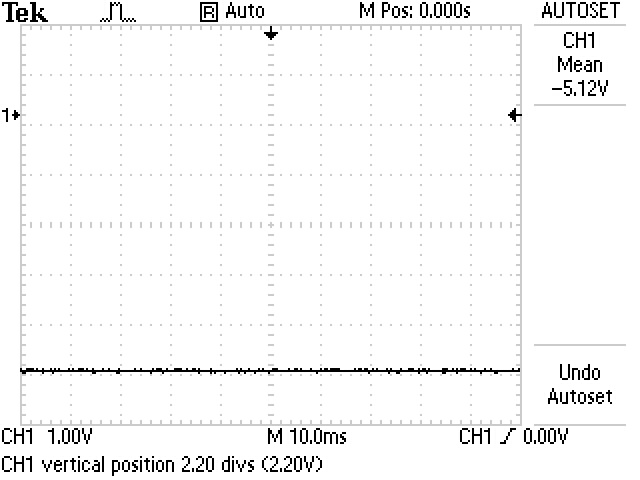
\includegraphics[width=1\linewidth]{./Figures/min_5V_output_voltage.JPG}
		    \caption{Charge pump output} \label{subfig:charge_pump_min_5V}
     \end{subfigure}
      \begin{subfigure}[]{0.45\textwidth}
              \centering
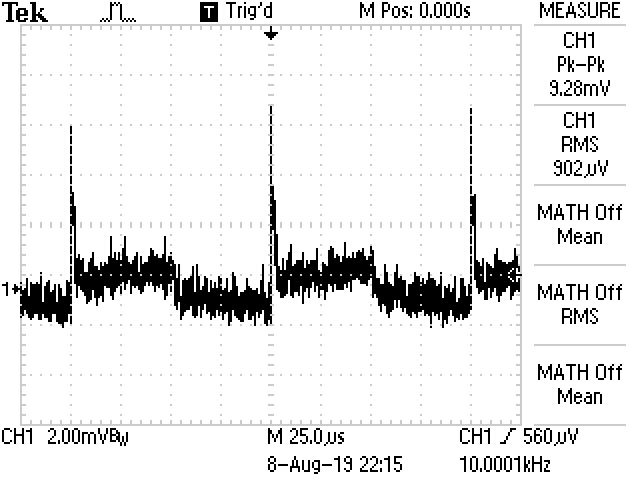
\includegraphics[width=1\linewidth]{./Figures/min_5V_output_noise.JPG}%
		    \caption{Noise characteristics}  \label{subfig:charge_pump_noise}
     \end{subfigure}
   \caption[Measured $\SI{-5}{V}$ Regulator Output Voltage Plots]{Measured $\SI{-5}{V}$ Regulator Output Voltage Plots. (a) reading showing output voltage, (b) output noise of the regulator}
    \label{fig:charge_pump_simulation_results_box}
 \end{figure}







